\documentclass[12pt,a4paper]{report}
\usepackage[utf8]{inputenc}
\usepackage[T1]{fontenc}
\usepackage{graphicx}
\usepackage{graphics}
\usepackage{fancyhdr}
\usepackage{geometry}
\usepackage{titlesec}
\usepackage{amsmath}
\usepackage{amsfonts}
\usepackage{amssymb}
\usepackage[french]{babel}
\usepackage{shadow}
\usepackage{latexsym}
\usepackage{marvosym}
\usepackage{enumerate}
\usepackage{xcolor}

\geometry{a4paper,
  left=20mm,
  right=20mm,
  top=30mm,
  bottom=30mm
}



\usepackage{listings}
\definecolor{codegreen}{rgb}{0,0.6,0}
\definecolor{codegray}{rgb}{0.5,0.5,0.5}
\definecolor{codepurple}{rgb}{0.58,0,0.82}
\definecolor{backcolour}{rgb}{0.95,0.95,0.92}

\lstdefinestyle{mystyle}{
    backgroundcolor=\color{backcolour},
    commentstyle=\color{codegreen},
    keywordstyle=\color{magenta},
    numberstyle=\tiny\color{codegray},
    stringstyle=\color{codepurple},
    basicstyle=\ttfamily\small,
    breakatwhitespace=false,
    breaklines=true,
    captionpos=b,
    keepspaces=true,
    numbers=left,
    numbersep=5pt,
    showspaces=false,
    showstringspaces=false,
    showtabs=false,
    tabsize=2
}

\lstset{style=mystyle}
\lstset{language=C}

\lstset{
literate=
{á}{{\'a}}1 {é}{{\'e}}1 {í}{{\'i}}1 {ó}{{\'o}}1 {ú}{{\'u}}1
{à}{{\`a}}1 {è}{{\`e}}1 {ì}{{\`i}}1 {ò}{{\`o}}1 {ù}{{\`u}}1
{€}{{\euro}}1 {ê}{{\^e}}1 {â}{{\^a}}1 {ô}{{\^o}}1
}


\begin{document}
\pagestyle{fancy}
	\renewcommand{\headrulewidth}{0.5pt}
	\fancyhead[R]{L3 Mathématiques et applications}
    \fancyhead[L]{ \leftmark}

\begin{titlepage}
  \begin{center}

    \LARGE
    \textbf{Université d'Évry Paris-Saclay}

    \vspace{1cm}

    \large
    Faculté des Sciences et Institut de Biologie Génétique et Bio-informatique

    \vspace{1cm}

    \large
    3ème année de Licence en Mathématiques et applications

    \vspace{1cm}


\includegraphics[scale=1]{logo_login.png} 
\includegraphics[scale=1]{Université_Paris_Saclay.png} 

    \vspace{1cm}

    \LARGE
    \textbf{Tetris}

    \vspace{1cm}

    \large
    Réalisé par :\\ SAMER Ahmed Wahid


    \vspace{1cm}

    \large
    Année académique : 2024 - 2025

  \end{center}
\end{titlepage}

\tableofcontents
    \thispagestyle{fancy}


\newpage
\chapter{Introduction}

\section{Contexte du projet}
Tetris, un jeu emblématique créé en 1985 par Alekseï Pajitnov, Dmitri Pavlovski et Vadim Guerassimov, a marqué l’histoire des jeux vidéo grâce à son gameplay simple et captivant. L’objectif principal du jeu est de manipuler des pièces géométriques appelées \emph{Tetriminos} pour former des lignes horizontales complètes, qui disparaissent lorsqu’elles sont remplies. Ce concept addictif a conduit à une popularité mondiale et à des adaptations sur presque toutes les plateformes.

\section{Objectif du projet}
Le projet vise à implémenter une version du jeu Tetris en respectant les spécifications essentielles du jeu original. Cela inclut :
\begin{itemize}
    \item le déplacement et la rotation des Tetriminos,
    \item la gestion du score et du niveau en fonction des lignes complétées,
    \item l’adaptation de la vitesse des Tetriminos selon le niveau atteint,
    \item l’affichage des statistiques du jeu telles que le score, le niveau, et les lignes détruites,
    \item l’utilisation de la bibliothèque SDL pour la partie graphique.
\end{itemize}
\section{Compilation du code}
Le sujet du projet impose que le code source soit compilé avec la commande suivante:

\begin{lstlisting}
$ gcc -g -O2 -Wall -Wextra -o tetris *.c $(pkg-config --cflags --libs sdl2 SDL2_ttf)
\end{lstlisting}

Cependant, dans notre implémentation, nous avons ajouté une fonctionnalité sonore en utilisant la bibliothèque \texttt{SDL2\_mixer}. Par conséquent, la commande de compilation a été modifiée pour inclure cette dépendance :

\begin{lstlisting}
$ gcc -g -O2 -Wall -Wextra -o Tetris *.c $(pkg-config --cflags --libs sdl2 SDL2_ttf SDL2_mixer)
\end{lstlisting}

Cette modification garantit une intégration fluide des éléments sonores.

\newpage
\chapter{Implémentation}

Le projet est organisé en plusieurs fichiers source et d’en-tête pour structurer le code et faciliter son développement. Voici un aperçu des principaux fichiers et leur rôle :

\section{Gestion des déplacements des Tetriminos}

\subsection{Représentation des Tetriminos}
Les Tetriminos sont représentés sous forme de tableaux 5×5, où chaque case contient une valeur indiquant la présence ou l'absence d'une partie du bloc. Par exemple, un Tetrimino de type \texttt{I} est représenté ainsi lorsqu'il n'est pas encore tourné :
\[
\begin{bmatrix}
0 & 0 & 0 & 0 & 0 \\
0 & 0 & 0 & 0 & 0 \\
0 & 1 & 1 & 1 & 1 \\
0 & 0 & 0 & 0 & 0 \\
0 & 0 & 0 & 0 & 0
\end{bmatrix}
\]
\begin{center}

\includegraphics[scale=1]{Fegure_I_Tetris.png} 
\end{center}

\subsection{Types de déplacements}
Les déplacements possibles sont :
\begin{itemize}
    \item \textbf{Vers la gauche} : réduire la colonne du Tetrimino.
    \item \textbf{Vers la droite} : augmenter la colonne du Tetrimino.
    \item \textbf{Vers le bas} : augmenter la ligne du Tetrimino.
\end{itemize}

Avant d'effectuer un déplacement, une vérification est effectuée pour s'assurer que la nouvelle position est valide (pas de collision avec un autre bloc ou un mur).

\subsection{Vérification des collisions}
La fonction de vérification des collisions, comme \texttt{tetris\_can\_go\_left}, parcourt chaque case du tableau \texttt{buffer} du Tetrimino. Si une case occupée par le Tetrimino entre en conflit avec un mur ou un bloc déjà fixé dans la matrice principale, le déplacement est annulé.

\paragraph{Exemple : Vérification à gauche}
\begin{lstlisting}
int tetris_can_go_left(Tetris *tet) {
    for (int i = 0; i < 5; i++) {
        for (int j = 0; j < 5; j++) {
            if (tet->buffer[i][j]) { // Case occupée
                int row = tet->current_line + i;
                int col = tet->current_column + j;
                // Si on est au bord gauche ou collision à gauche
                if (col == 0 || tet->matrix[row][col - 1] != 0) {
                    return 0; // Déplacement impossible
                }
            }
        }
    }
    return 1; // Déplacement possible
}
\end{lstlisting}

\subsection{Implémentation des déplacements}
Les fonctions de déplacement, comme \texttt{tetris\_move\_left}, modifient les coordonnées du Tetrimino si le déplacement est valide.

\paragraph{Exemple : Déplacement à gauche}
\begin{lstlisting}
void tetris_move_left(Tetris *tet) {
    if (tetris_can_go_left(tet)) {
        tet->current_column--; // Déplace le Tetrimino d'une colonne à gauche
    }
}
\end{lstlisting}

De manière similaire, les déplacements vers la droite (\texttt{tetris\_move\_right}) et vers le bas (\texttt{tetris\_move\_down}) suivent le même principe, mais en adaptant la vérification des collisions et la mise à jour des coordonnées.
\newpage

\section{Gestion des rotations des Tetriminos}

\subsection{Principe de la rotation}
Les Tetriminos peuvent pivoter contre le sens des aiguilles d'une montre. Cette opération est réalisée en transposant leur tableau 5×5, puis en inversant les colonnes. Par exemple, une rotation de 90\textdegree{} du Tetrimino \texttt{T} passe de cette forme initiale :
\[
\begin{bmatrix}
0 & 0 & 0 & 0 & 0 \\
0 & 0 & 6 & 0 & 0 \\
0 & 0 & 6 & 6 & 0 \\
0 & 0 & 6 & 0 & 0 \\
0 & 0 & 0 & 0 & 0
\end{bmatrix}
\]
\begin{center}

\includegraphics[scale=1]{FIgure_T_inv_Tetris.png} 
\end{center}
à :
\[
\begin{bmatrix}
0 & 0 & 0 & 0 & 0 \\
0 & 0 & 6 & 0 & 0 \\
0 & 6 & 6 & 6 & 0 \\
0 & 0 & 0 & 0 & 0 \\
0 & 0 & 0 & 0 & 0
\end{bmatrix}
\]
\begin{center}

\includegraphics[scale=1]{Fegure_T_Tetris.png} 
\end{center}

\newpage
\subsection{Vérification de la validité de la rotation}
Avant d’appliquer une rotation, une vérification est nécessaire pour s'assurer que :
\begin{itemize}
    \item La nouvelle position du Tetrimino ne dépasse pas les limites de la matrice.
    \item La rotation ne provoque pas de collision avec d'autres blocs.
\end{itemize}

Cette vérification est réalisée par la fonction \texttt{tetris\_is\_valid\_position}, qui vérifie chaque case du tableau après rotation.

\paragraph{Exemple : Validation d'une rotation}
\begin{lstlisting}
int tetris_is_valid_position(Tetris *tet, char new_buffer[5][5]) {
    for (int i = 0; i < 5; i++) {
        for (int j = 0; j < 5; j++) {
            if (new_buffer[i][j]) { // Case occupée
                int row = tet->current_line + i;
                int col = tet->current_column + j;
                // Vérification des limites
                if (row < 0 || row >= 20 || col < 0 || col >= 10) return 0; // Hors limites
                // Vérification des collisions
                if (tet->matrix[row][col]) return 0; // Collision détectée
            }
        }
    }
    return 1; // Rotation valide
}
\end{lstlisting}

\subsection{Implémentation de la rotation}
La rotation est gérée par cette fonction:
\begin{itemize}
    \item \textbf{\texttt{tetris\_rotate}} : Effectue la rotation en modifiant le tableau \texttt{buffer} si elle est valide.
\end{itemize}

\paragraph{Exemple : Application de la rotation}
\begin{lstlisting}
void tetris_rotate(Tetris *tet) {
    int new_rotation = (tet->current_rotation + 1) % 4;
    char new_buffer[5][5] = {0};
    for (int i = 0; i < 5; i++) {
        for (int j = 0; j < 5; j++) {
            new_buffer[j][4 - i] = tetriminos[tet->current_type][new_rotation][i][j];
        }
    }
    if (tetris_is_valid_position(tet, new_buffer)) {
        memcpy(tet->buffer, new_buffer, sizeof(new_buffer));
        tet->current_rotation = new_rotation;
    }
}
\end{lstlisting}

\newpage

\section{Calcul du score et des niveaux}

\subsection{Principe général}
Le score et les niveaux sont des mécanismes clés pour récompenser le joueur et augmenter la difficulté progressivement. Chaque fois qu’une ou plusieurs lignes sont complétées, elles sont supprimées, et un score est attribué en fonction du nombre de lignes éliminées simultanément.

\subsection{Calcul du score}
Le score est calculé selon une formule qui dépend du nombre de lignes détruites en une seule fois et du niveau actuel du joueur. Plus il y a de lignes éliminées simultanément, plus la récompense est importante.

\textbf{Table des points} :
\[
\text{Score} = \text{multiplicateur} \times \text{niveau}
\]
où le multiplicateur dépend du nombre de lignes détruites :
\begin{itemize}
    \item 1 ligne : \(100\)
    \item 2 lignes : \(300\)
    \item 3 lignes : \(500\)
    \item 4 lignes : \(800\) (appelé un "Tetris").
\end{itemize}

\textbf{Exemple} : Un joueur au niveau 3 qui détruit 2 lignes obtiendra \(300 \times 3 = 900\) points.

\paragraph{Extrait de code : Gestion des points}
\begin{lstlisting}
if (lines_cleared > 0) {
    tet->nbr_lines += lines_cleared; // Mise à jour des lignes totales

    switch (lines_cleared) {
        case 1:
            tet->score += 100 * tet->level;
            break;
        case 2:
            tet->score += 300 * tet->level;
            break;
        case 3:
            tet->score += 500 * tet->level;
            break;
        case 4: // "Tetris"
            tet->score += 800 * tet->level;
            break;
        default:
            // Rare, au cas où plus de 4 lignes sont détruites simultanément
            tet->score += 800 * tet->level;
            break;
    }
}
\end{lstlisting}

\subsection{Gestion des niveaux}
Le niveau du joueur augmente au fur et à mesure qu’il progresse dans le jeu. Chaque fois que le joueur élimine un total de 10 lignes, le niveau augmente de 1, jusqu’à un maximum de 15.

\paragraph{Extrait de code : Mise à jour du niveau}
\begin{lstlisting}
while (tet->nbr_lines >= 10) {
    tet->nbr_lines -= 10; // Réinitialise les lignes comptabilisées pour le niveau actuel
    tet->level++;
    if (tet->level > 15) {
        tet->level = 15; // Niveau maximal
        break;
    }
}
\end{lstlisting}

\subsection{Vitesse de descente des Tetriminos}
Avec chaque niveau, la vitesse à laquelle les Tetriminos descendent augmente. Cette vitesse est calculée à l’aide d’une formule :
\[
\text{vitesse} = 0.8 - (0.007 \times (\text{niveau} - 1))^{\text{niveau} - 1}
\]
À partir du niveau 15, la vitesse est fixée à \(0.007\) seconde par ligne.

\textbf{Table approximative des vitesses} :
\[
\begin{array}{|c|c|}
\hline
\text{Niveau} & \text{Vitesse (secondes par ligne)} \\
\hline
1 & 1.0 \\
5 & 0.355 \\
10 & 0.064 \\
15 & 0.007 \\
\hline
\end{array}
\]

\paragraph{Extrait de code : Calcul de la vitesse}
\begin{lstlisting}
float tetris_get_drop_speed(Tetris *tet) {
    int l = tet->level;
    if (l < 1) l = 1;
    if (l > 15) l = 15;

    float base = 0.8f - ((l - 1) * 0.007f);
    if (base < 0.0f) base = 0.0f;

    float speed = powf(base, (float)(l - 1));
    return speed < 0.007f ? 0.007f : speed; // Minimum 0.007
}
\end{lstlisting}
\newpage

\section{L’affichage graphique avec SDL}

\subsection{Initialisation de SDL}
L'initialisation de SDL configure la fenêtre, le renderer, et les polices nécessaires pour l'affichage du jeu. Cette étape est essentielle pour établir l'environnement graphique. Le code ci-dessous montre les étapes principales, comme la création d'une fenêtre et d'un renderer.

\begin{lstlisting}
// Initialisation de SDL pour la vidéo
if (SDL_Init(SDL_INIT_VIDEO) != 0) {
    fprintf(stderr, "Erreur SDL_Init: %s\n", SDL_GetError());
    return 0;
}

// Création de la fenêtre de jeu
g->win = SDL_CreateWindow("Tetris", x, y, 500, 600, SDL_WINDOW_SHOWN);
if (!g->win) {
    fprintf(stderr, "Erreur SDL_CreateWindow\n");
    return 0;
}

// Création du renderer pour gérer le dessin
g->ren = SDL_CreateRenderer(g->win, -1, SDL_RENDERER_ACCELERATED | SDL_RENDERER_PRESENTVSYNC);
if (!g->ren) {
    fprintf(stderr, "Erreur SDL_CreateRenderer\n");
    return 0;
}

// Initialisation des polices pour le texte
g->fontSmall = TTF_OpenFont("Tetris.ttf", 14);
g->fontLarge = TTF_OpenFont("Tetris.ttf", 64);

// Initialisation de l'audio pour les effets sonores
if (Mix_OpenAudio(44100, MIX_DEFAULT_FORMAT, 2, 2048) < 0) {
    fprintf(stderr, "Erreur Mix_OpenAudio\n");
    return 0;
}
\end{lstlisting}

Dans cet exemple, on remarque l'utilisation des bibliothèques SDL pour la gestion des fenêtres, des polices et des sons. Chaque étape vérifie les erreurs pour s'assurer que le jeu peut continuer à s'exécuter.
\newpage


\subsection{Affichage du plateau de jeu}
Le plateau est une matrice de 10 colonnes et 20 lignes. Les Tetriminos fixés et en mouvement sont affichés séparément pour garantir une distinction visuelle claire.

\paragraph{Affichage des blocs fixés}
Les blocs déjà placés dans la matrice principale sont parcourus et affichés en fonction de leur type.

\begin{lstlisting}
// Dessin du cadre du plateau
SDL_Rect game_frame = {0, 0, 300, 600};
SDL_SetRenderDrawColor(g->ren, 255, 0, 255, 255);
SDL_RenderDrawRect(g->ren, &game_frame);

// Dessin de l'arrière-plan des stats
SDL_Rect stats_bg = {300, 0, 200, 600};
SDL_SetRenderDrawColor(g->ren, 30, 30, 30, 255);
SDL_RenderFillRect(g->ren, &stats_bg);
        
for (int i = 0; i < 20; i++) {
    for (int j = 0; j < 10; j++) {
        if (g->tet->matrix[i][j] != 0) {
            // Affichage d'un bloc (fixé) en fonction de sa position
            mino_display(g, g->tet->matrix[i][j] - 1, i, j);
        }
    }
}
\end{lstlisting}

\paragraph{Affichage des Tetriminos en mouvement}
Les Tetriminos en mouvement sont affichés en utilisant leur position actuelle dans le buffer.

\begin{lstlisting}
for (int i = 0; i < 5; i++) {
    for (int j = 0; j < 5; j++) {
        if (g->tet->buffer[i][j] != 0) {
            // Calcul des coordonnées absolues
            int row = g->tet->current_line + i;
            int col = g->tet->current_column + j;
            // Affichage du bloc correspondant
            mino_display(g, g->tet->current_type, row, col);
        }
    }
}
\end{lstlisting}

\newpage
\subsection{Affichage des statistiques}
Les statistiques du jeu (score, niveau, lignes détruites) sont affichées sur une section dédiée de la fenêtre, à droite du plateau. Une prévisualisation du prochain Tetrimino est également fournie pour aider le joueur à planifier ses mouvements.

\paragraph{Affichage du score}
\begin{lstlisting}
// Affichage du score du joueur
snprintf(info, sizeof(info), "Score: %d", g->tet->score);
surface = TTF_RenderText_Solid(g->fontSmall, info, color);
texture = SDL_CreateTextureFromSurface(g->ren, surface);
rect = (SDL_Rect){325, 50, surface->w, surface->h};
SDL_RenderCopy(g->ren, texture, NULL, &rect);
SDL_FreeSurface(surface);
SDL_DestroyTexture(texture);
\end{lstlisting}

\paragraph{Prévisualisation du prochain Tetrimino}
La prévisualisation affiche le Tetrimino suivant dans une petite zone à droite.

\begin{lstlisting}
SDL_Rect preview_frame = {325, 200, 150, 150};
SDL_SetRenderDrawColor(g->ren, 255, 0, 255, 255);
SDL_RenderDrawRect(g->ren, &preview_frame);
for (int i = 0; i < 5; i++)
{
    for (int j = 0; j < 5; j++)
    {
        if (tetriminos[g->tet->next_type][0][i][j])
        {
            // Coordonnées du mini-bloc
            SDL_Rect block = {
                preview_frame.x + j * 30,
                preview_frame.y + i * 30,
                27, 27};

            // Récupère la couleur de base du Tetrimino
            Color base = TetriminoColors[g->tet->next_type];
            Color light = {
                base.r + 50 > 255 ? 255 : base.r + 50,
                base.g + 50 > 255 ? 255 : base.g + 50,
                base.b + 50 > 255 ? 255 : base.b + 50};
            Color dark = {
                base.r - 50 < 0 ? 0 : base.r - 50,
                base.g - 50 < 0 ? 0 : base.g - 50,
                base.b - 50 < 0 ? 0 : base.b - 50};

            // Peins le bloc avec la couleur de base
            SDL_SetRenderDrawColor(g->ren, base.r, base.g, base.b, 255);
            SDL_RenderFillRect(g->ren, &block);

            // Ajoute la bande claire (en haut)
            SDL_SetRenderDrawColor(g->ren, light.r, light.g, light.b, 255);
            SDL_Rect top_band = {block.x, block.y, (3 * block.w) / 4, block.h / 4};
            SDL_RenderFillRect(g->ren, &top_band);

            // Ajoute la bande claire (à gauche)
            SDL_Rect left_band = {block.x, block.y, block.w / 4, (3 * block.h) / 4};
            SDL_RenderFillRect(g->ren, &left_band);

            // Ajoute la bande sombre (en bas)
            SDL_SetRenderDrawColor(g->ren, dark.r, dark.g, dark.b, 255);
            SDL_Rect bottom_band = {block.x, block.y + (3 * block.h) / 4, block.w, block.h / 4 + 1};
            SDL_RenderFillRect(g->ren, &bottom_band);

            // Ajoute la bande sombre (à droite)
            SDL_Rect right_band = {block.x + (3 * block.w) / 4, block.y, block.w / 4 + 1, block.h};
            SDL_RenderFillRect(g->ren, &right_band);
        }
    }
}
\end{lstlisting}
\newpage
\subsection{Gestion des états du jeu}
L’affichage change en fonction de l’état du jeu : menu principal, jeu en cours, pause ou fin de partie.

\paragraph{Exemple : Écran "Game Over"}
\begin{lstlisting}
case STATE_GAMEOVER:
{
    // Affichage du message "Game Over"
    SDL_Color color1 = {255, 0, 0, 255}; // Rouge
    SDL_Surface *surface = TTF_RenderText_Solid(g->fontLarge, "GAME OVER", color1);
    SDL_Texture *texture = SDL_CreateTextureFromSurface(g->ren, surface);
    SDL_Rect dstRect;
    dstRect.x = (500 - surface->w) / 2;
    dstRect.y = (600 - surface->h) / 4;
    dstRect.w = surface->w;
    dstRect.h = surface->h;
    SDL_RenderCopy(g->ren, texture, NULL, &dstRect);
    SDL_FreeSurface(surface);
    SDL_DestroyTexture(texture);
    /*..................*/
}
\end{lstlisting}

\subsection{Boucle de rendu}
La boucle de rendu rafraîchit l’écran pour refléter les changements dans l’état du jeu.

\begin{lstlisting}
void game_update(Game *g) {
    SDL_SetRenderDrawColor(g->ren, 24, 24, 24, 255);
    SDL_RenderClear(g->ren);
    switch (g->state) {
        case STATE_MENU:
            // Affichage du menu principal
            break;
        case STATE_PLAY:
            // Dessin du plateau et des statistiques
            break;
        case STATE_GAMEOVER:
            // Affichage de l'écran "Game Over"
            break;
        case STATE_PAUSE:
            // Affichage de l'écran de pause
            break;
    }
    SDL_RenderPresent(g->ren);
}
\end{lstlisting}

\newpage
\section{La gestion des entrées utilisateur}

\subsection{Principe général}
Dans Tetris, les entrées utilisateur permettent d’interagir avec le jeu en déplaçant les Tetriminos, en les faisant pivoter, ou en contrôlant la vitesse de leur descente. Ces entrées sont gérées via les événements détectés par SDL dans une boucle d’événements.

Les actions principales gérées par les entrées utilisateur sont :
\begin{itemize}
    \item \textbf{Déplacement gauche/droite} : Déplacer le Tetrimino horizontalement.
    \item \textbf{Descente rapide} : Accélérer la descente du Tetrimino.
    \item \textbf{Rotation} : Pivoter le Tetrimino.
    \item \textbf{Pause ou Quitter le jeu} : Gérer des états comme la pause ou l’arrêt du jeu.
\end{itemize}

\subsection{Gestion des événements SDL}
SDL capture les événements utilisateur (comme les appuis sur des touches) via la fonction \texttt{SDL\_PollEvent}. Chaque événement est ensuite analysé pour déterminer quelle action doit être effectuée.

\paragraph{Exemple : Gestion des touches}
\begin{lstlisting}
SDL_Event e;
while (SDL_PollEvent(&e)) {
    // Si l'utilisateur ferme la fenêtre
    if (e.type == SDL_QUIT) {
        running = 0; // Arrêter la boucle du jeu
    }
    // Si une touche est appuyée
    else if (e.type == SDL_KEYDOWN) {
        switch (e.key.keysym.sym) {
            case SDLK_LEFT: // Flèche gauche
                tetris_move_left(g->tet);
                break;
            case SDLK_RIGHT: // Flèche droite
                tetris_move_right(g->tet);
                break;
            case SDLK_DOWN: // Flèche bas
                tetris_move_down(g->tet);
                break;
            case SDLK_UP: // Flèche haut
                tetris_rotate(g->tet);
                break;
            case SDLK_p: // Pause
                g->state = (g->state == STATE_PLAY) ? STATE_PAUSE : STATE_PLAY;
                break;
            case SDLK_ESCAPE: // Quitter
                running = 0;
                break;
            default:
                break;
        }
    }
}
\end{lstlisting}

\subsection{Implémentation des actions}
Chaque action correspond à une fonction spécifique :
\begin{itemize}
    \item \textbf{Déplacement à gauche/droite} : \texttt{tetris\_move\_left} et \texttt{tetris\_move\_right} mettent à jour la position du Tetrimino.
    \item \textbf{Rotation} : \texttt{tetris\_rotate} applique une rotation si elle est valide.
    \item \textbf{Descente rapide} : \texttt{tetris\_move\_down} accélère la descente du Tetrimino en mettant à jour sa position plus fréquemment.
\end{itemize}

\paragraph{Exemple : Rotation avec \texttt{SDL\_KEYDOWN}}
\begin{lstlisting}
case SDLK_UP: // Flèche haut
    if (tetris_can_rotate(g->tet)) { // Vérifie si la rotation est possible
        tetris_rotate(g->tet);       // Effectue la rotation
    }
    break;
\end{lstlisting}

\subsection{Gestion des états (Pause et Quitter)}
Des touches spécifiques permettent de gérer l’état global du jeu :
\begin{itemize}
    \item \textbf{Pause} : La touche \texttt{p} bascule entre les états \texttt{STATE\_PLAY} et \texttt{STATE\_PAUSE}.
    \item \textbf{Quitter} : La touche \texttt{ESC} arrête le jeu en mettant fin à la boucle principale.
\end{itemize}

\paragraph{Exemple : Pause}
\begin{lstlisting}
case SDLK_p: // Pause
    if (g->state == STATE_PLAY) {
        g->state = STATE_PAUSE;      // Mettre en pause
        Mix_HaltMusic();             // Arrêter la musique de fond
    } else if (g->state == STATE_PAUSE) {
        g->state = STATE_PLAY;       // Reprendre le jeu
        Mix_PlayMusic(g->music, -1); // Relancer la musique
    }
    break;
\end{lstlisting}

\newpage
\subsection{Synchronisation avec la boucle principale}
Les entrées utilisateur sont synchronisées avec la boucle principale du jeu. Chaque action est appliquée immédiatement et l’écran est mis à jour en conséquence via la fonction \texttt{game\_update}.

\paragraph{Exemple : Synchronisation dans la boucle}
\begin{lstlisting}
while (running) {
    // Gestion des événements utilisateur

    // Mise à jour de l'état du jeu
    if (g->state == STATE_PLAY) {
        game_update(g);
    }
}
\end{lstlisting}

\section{Fin de partie}

\subsection{Détection de la fin de partie}
La fin de partie dans Tetris est détectée lorsqu’un Tetrimino ne peut pas être placé en haut de la matrice, car la première ligne est déjà occupée par des blocs fixés. Cela se produit lorsque le joueur n’a pas réussi à éliminer suffisamment de lignes.

\paragraph{Exemple : Matrice bloquée}
Voici un exemple où un nouveau Tetrimino ne peut pas être placé, déclenchant ainsi la fin de la partie :
\\
\begin{center}
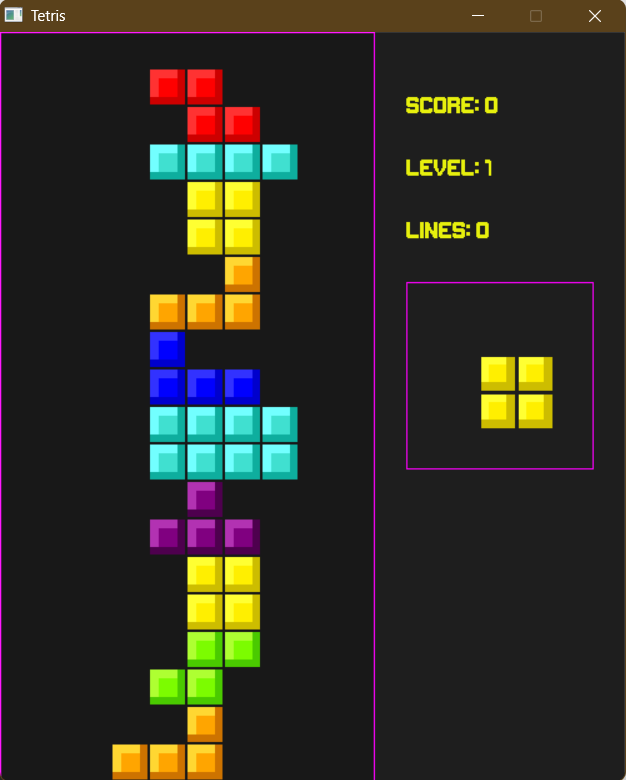
\includegraphics[scale=0.5]{Figure_Presque.png} 
\end{center}
\\

\subsection{Implémentation}
La vérification de la fin de partie est réalisée par la fonction suivante, S'il ne peut pas descendre ET qu'il est tout en haut dans la fonction tetris move down:
\\
\begin{lstlisting}
if (tet->current_line == 0)
{
    return -1;
}
\end{lstlisting}

\subsection{Affichage de l'écran "Game Over"}
Lorsqu’une fin de partie est détectée, un écran dédié s’affiche avec le message "GAME OVER", des instructions pour rejouer ou quitter, ainsi que les statistiques finales du joueur.

\paragraph{Statistiques finales affichées :}
\begin{itemize}
    \item \textbf{Score final} : Affiche le score obtenu par le joueur.
    \item \textbf{Niveau atteint} : Indique le niveau final du joueur.
    \item \textbf{Lignes détruites} : Montre le nombre total de lignes supprimées.
\end{itemize}

\subsection{Relancer ou quitter la partie}
Après la fin de la partie, le joueur peut choisir de relancer une nouvelle partie ou de quitter le jeu. Ces actions sont gérées via des entrées clavier :
\begin{itemize}
    \item Appuyer sur \texttt{ESPACE} ou \texttt{ENTRÉE} pour relancer la partie.
    \item Appuyer sur \texttt{ESC} pour quitter le jeu.
\end{itemize}

\paragraph{Exemple : Gestion des entrées après la fin}
\begin{lstlisting}
if (g->state == STATE_GAMEOVER) {
    switch (e.key.keysym.sym) {
        case SDLK_SPACE:
        case SDLK_RETURN:
            memset(g->tet->matrix, 0, sizeof(g->tet->matrix));
            g->tet->score = 0;
            g->tet->nbr_lines = 0;
            tetris_reset(g->tet);
            g->state = STATE_PLAY; // Revenir à l'état de jeu
            break;
        case SDLK_ESCAPE:
            running = 0; // Quitter le jeu
            break;
    }
}
\end{lstlisting}

\newpage



\chapter{Problèmes rencontrés}

\section{Problèmes rencontrés et solutions}

\subsection{Absence de chiffres dans la police utilisée}
\paragraph{Problème :} 
Au début, la police utilisée pour afficher les textes (\texttt{Tetris.ttf}) ne contenait pas de chiffres. Cela empêchait l’affichage des informations essentielles, comme le score, le niveau, et le nombre de lignes détruites.\\
\begin{center}

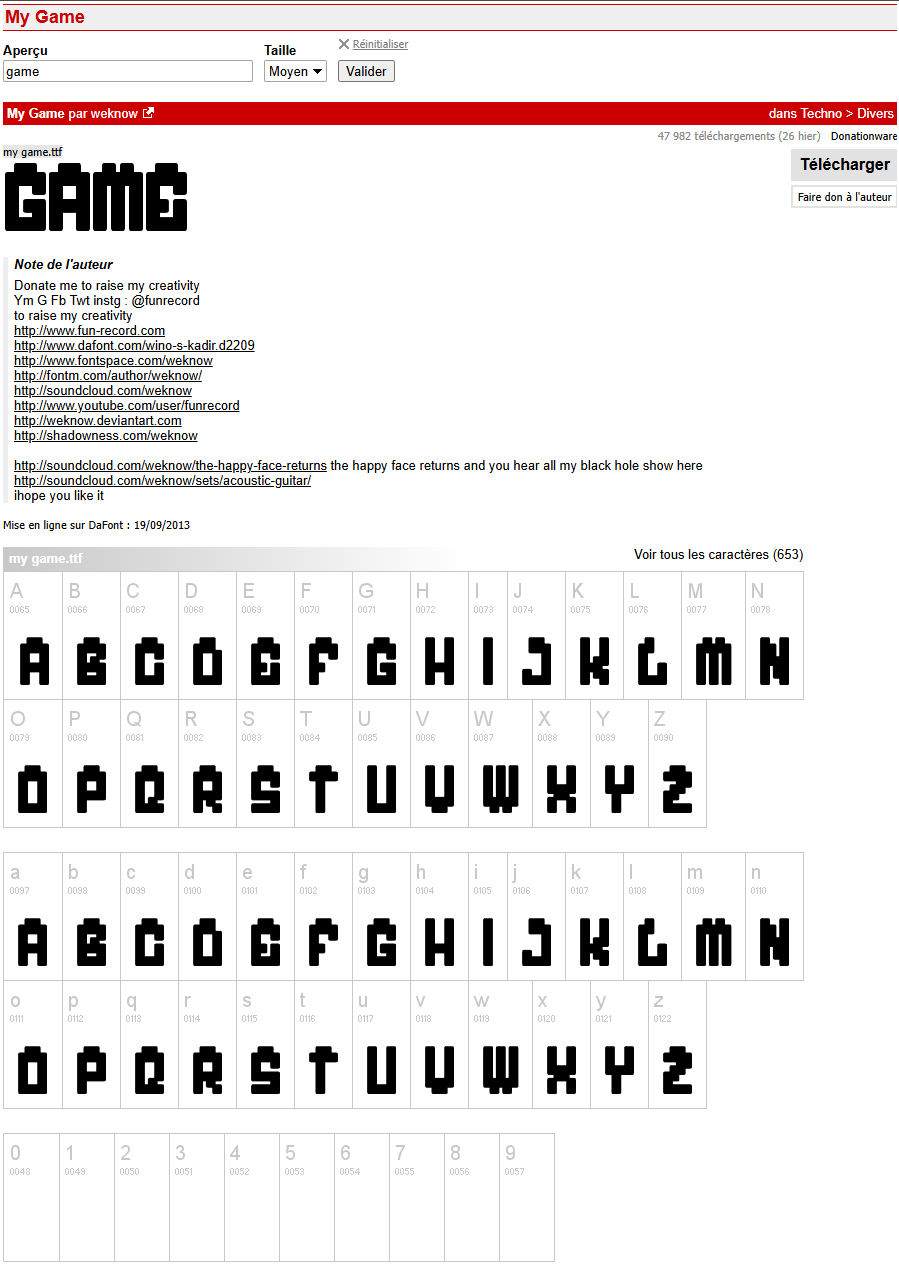
\includegraphics[scale=0.35]{Figure_My_Game.png} 
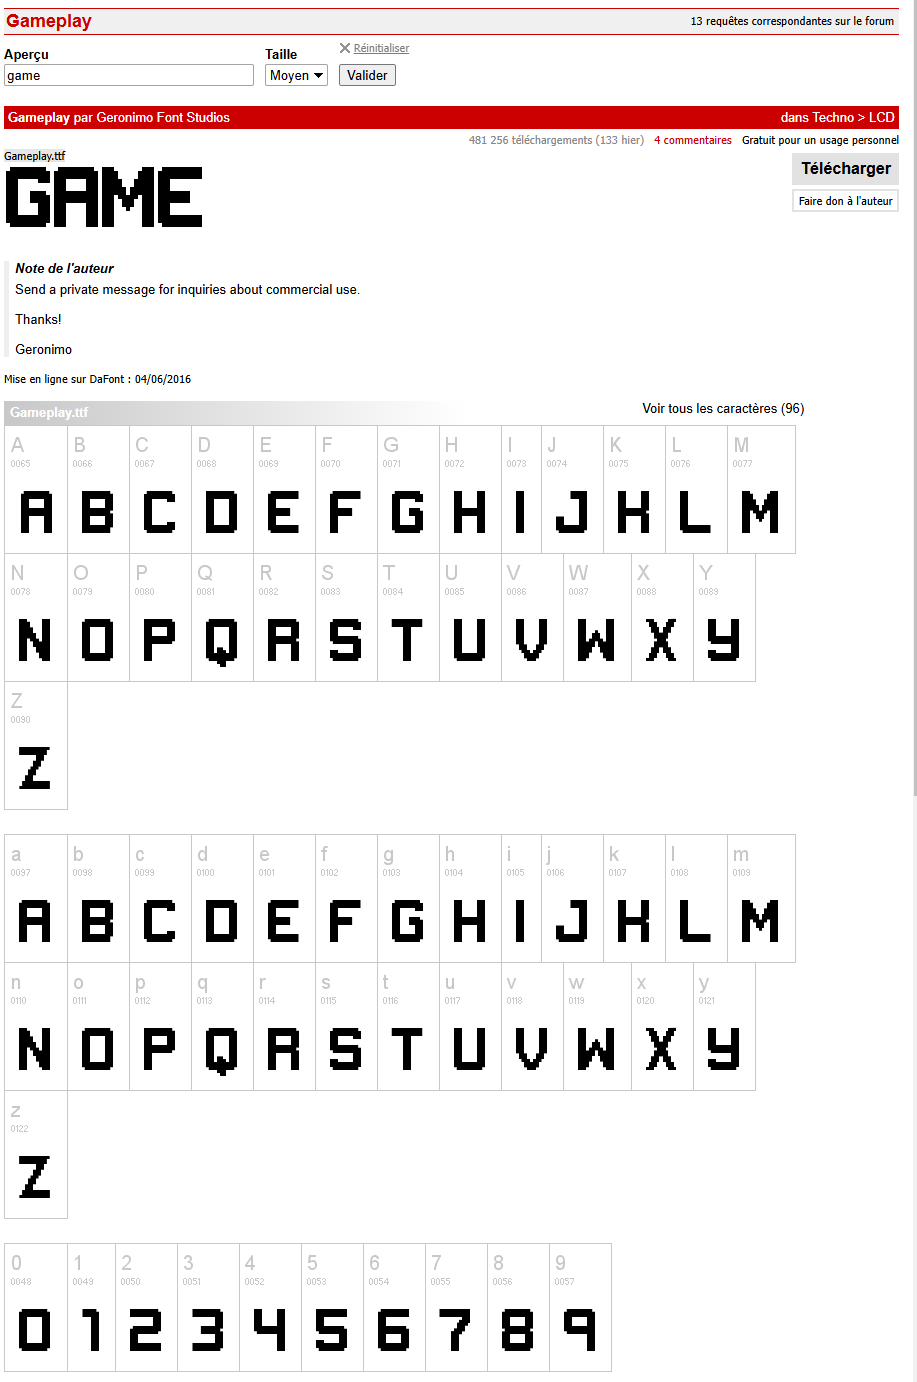
\includegraphics[scale=0.35]{Figure_GAMEPLAY.png} 

\end{center}
\\
\paragraph{Solution :}
Une nouvelle police a été téléchargée et intégrée dans le projet, permettant d’afficher correctement toutes les informations. Les modifications ont porté sur le fichier où la police était initialisée.

\subsection{Blocs stagnants en haut du plateau}
\paragraph{Problème :}
Certains Tetriminos apparaissaient en haut du plateau mais restaient immobiles, sans descendre comme prévu. Cela bloquait le déroulement normal du jeu.
\\
\begin{center}

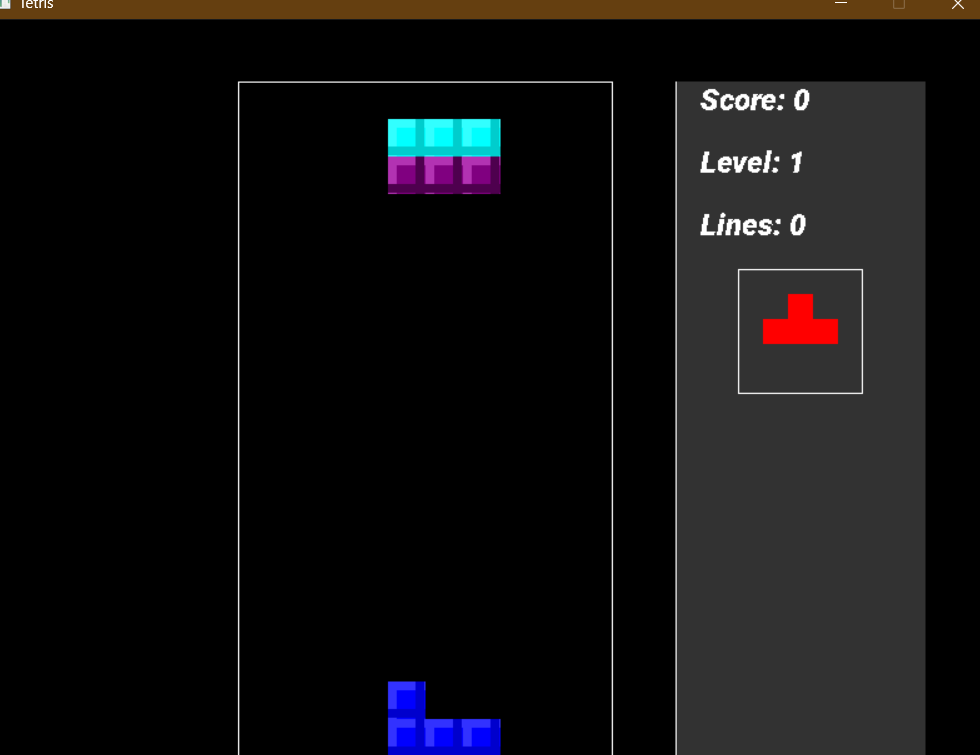
\includegraphics[scale=0.5]{Figure_Bloque.png} 

\end{center}
\\
\paragraph{Solution :}
Ce problème était lié à un bug dans la logique de descente des Tetriminos. En corrigeant les appels à la fonction de descente et en vérifiant les conditions de collision dans la matrice, les Tetriminos ont repris leur mouvement dès leur apparition.
\\
\subsection{Segmentation fault imprévisible}
\paragraph{Problème :}
Une erreur de segmentation survenait aléatoirement pendant l’exécution, mais elle semblait se résoudre d’elle-même après certaines modifications dans le code.

\paragraph{Solution :}
Bien que ce problème n’ait pas été réglé explicitement, la cause était probablement liée à des indices de matrice invalides. Après avoir corrigé d’autres parties du code, le problème a disparu.
\newpage

\subsection{Game Over non détecté}
\paragraph{Problème :}
Lorsque les blocs atteignaient le sommet du plateau, le jeu continuait à générer de nouveaux Tetriminos au lieu de détecter la fin de partie. Cela rendait le jeu infini et bloquait l'utilisateur.
\\

\begin{lstlisting}
int tetris_move_down(Tetris *tet)
{
    // Peut-on descendre ?
    if (tetris_can_go_down(tet))
    {
        tet->current_line++;
        return 1; // Succès : on a bougé
    }
    else
    {
        // S'il ne peut pas descendre ET qu'il est tout en haut
        // => Game Over (on renvoie un code spécial, disons -1)
        if (tet->current_line == 0)
        {
            // La pièce n'a jamais pu bouger => bloqué dès le spawn
            return -1;
        }

        // Sinon, c'est juste la fin de la descente (on fixe la pièce)
        tetris_shift_board(tet);
        tetris_reset(tet);

        return 0; // "J'ai fini, mais pas de Game Over"
    }
}
\end{lstlisting}

\\
\paragraph{Solution :}
la fonction tetris move down a été corrige pour vérifier s'il ne peut pas descendre et qu'il est tout en haut. l’état du jeu passe à \texttt{STATE\_GAMEOVER}.


\newpage
\chapter{Choix techniques et justifications}

\section{Utilisation d'un buffer \(5 \times 5\) au lieu de \(20 \times 10\)}

\paragraph{Problème et contexte :}
Dans les spécifications du projet, il était mentionné d’utiliser une matrice de buffer de \(20 \times 10\) pour gérer les déplacements et les collisions des Tetriminos. Cependant, dans ce projet, un buffer de \(5 \times 5\) a été utilisé pour les Tetriminos en mouvement. Ce choix diffère de la spécification originale, mais il s'avère plus adapté pour certains aspects de la gestion des Tetriminos.

\subsection{Avantages d’un buffer \(5 \times 5\)}
\begin{itemize}
    \item \textbf{Simplicité de gestion :} Un buffer de \(5 \times 5\) correspond exactement à la taille maximale d’un Tetrimino, peu importe sa rotation. Cela facilite les calculs et les vérifications.
    \item \textbf{Optimisation mémoire :} Le buffer de \(5 \times 5\) utilise beaucoup moins de mémoire que celui de \(20 \times 10\). Comme il ne contient que le Tetrimino en mouvement, il n’a pas besoin de refléter toute la matrice de jeu.
    \item \textbf{Clarté du code :} Les fonctions comme \texttt{tetris\_can\_go\_down} ou \texttt{tetris\_can\_rotate} n’ont besoin de parcourir que \(5 \times 5 = 25\) cases, au lieu de \(20 \times 10 = 200\) cases.
\end{itemize}

\subsection{Implémentation}
Le buffer \(5 \times 5\) est utilisé pour stocker le Tetrimino en cours de mouvement. Les calculs de collisions et de positions sont effectués en utilisant ce buffer.

\paragraph{Déclaration du buffer :}
\begin{lstlisting}
typedef struct {
    char matrix[20][10]; // Matrice des blocs fixés
    char buffer[5][5];   // Buffer pour le Tetrimino en mouvement
    ...
} Tetris;
\end{lstlisting}
\newpage
\paragraph{Utilisation dans les fonctions :}
Les fonctions comme \texttt{tetris\_can\_go\_down} et \texttt{tetris\_rotate} utilisent le buffer \(5 \times 5\) pour gérer les déplacements et les rotations.

\begin{lstlisting}
// Exemple : Vérification de la descente
int tetris_can_go_down(Tetris *tet) {
    for (int i = 0; i < 5; i++) {
        for (int j = 0; j < 5; j++) {
            if (tet->buffer[i][j]) { // Case occupée
                int row = tet->current_line + i;
                int col = tet->current_column + j;
                // Vérification des limites et collisions
                if (row == 19 || tet->matrix[row + 1][col] != 0) {
                    return 0; // Descente impossible
                }
            }
        }
    }
    return 1; // Descente possible
}
\end{lstlisting}

\subsection{Limites de ce choix}
\begin{itemize}
    \item \textbf{Calculs supplémentaires :} Les coordonnées globales du Tetrimino doivent être recalculées à chaque vérification, car le buffer \(5 \times 5\) n'est pas aligné avec la matrice \(20 \times 10\).
\end{itemize}

\newpage
\section{Affichage des Minos et Raffinements esthétiques}

\subsection{Choix des dimensions des bandes de relief}
Dans notre projet, la fonction \texttt{mino\_display} est responsable de l'affichage des Minos avec un effet de relief, obtenu grâce à l'utilisation de bandes claire et sombre. Les spécifications initiales du projet proposaient des bandes très minces, reflétant un rendu discret (comme indiqué dans le sujet). Cependant, nous avons choisi de privilégier des reliefs plus épais pour donner un effet visuel plus immersif et captivant.
\\

Deux configurations principales ont été testées :
\begin{itemize}
\item \textbf{Proportions \texttt{(7 * size) / 8} et \texttt{size / 8} :} Ce rendu donne un effet élégant et équilibré, avec des reliefs minces qui rappellent une approche minimaliste.
\item \textbf{Proportions \texttt{(3 * size) / 4} et \texttt{size / 4} :} Ce choix, finalement adopté, offre des reliefs plus épais, évoquant des bonbons translucides ou des émeraudes. Nous avons préféré cette approche car elle apporte une touche distinctive et accrocheuse au design.
\end{itemize}

\subsection{Ajustements des proportions et impact visuel}

Voici le code de la fonction \texttt{mino\_display} :
\begin{lstlisting}
void mino_display(Game *g, Type t, int l, int c)
{   /*.............*/
    // Couleur de base (plein du mino)
    SDL_SetRenderDrawColor(g->ren, base.r, base.g, base.b, 0xFF);
    rect = (SDL_Rect){x, y, (3 * size) / 4, (3 * size) / 4};
    SDL_RenderFillRect(g->ren, &rect);
    
    // Ligne supérieure (claire)
    SDL_SetRenderDrawColor(g->ren, light.r, light.g, light.b, 0xFF);
    rect = (SDL_Rect){x, y, (3 * size) / 4, size / 4};
    SDL_RenderFillRect(g->ren, &rect);
    // Colonne gauche (claire)
    
    rect = (SDL_Rect){x, y, size / 4, (3 * size) / 4};
    SDL_RenderFillRect(g->ren, &rect);
    // Ligne inférieure (sombre)
    
    SDL_SetRenderDrawColor(g->ren, dark.r, dark.g, dark.b, 0xFF);
    rect = (SDL_Rect){x, y + (3 * size) / 4, size - 2, size / 4 - 1};
    SDL_RenderFillRect(g->ren, &rect);
    // Colonne droite (sombre)
    
    rect = (SDL_Rect){x + (3 * size) / 4, y, size / 4 - 1, size - 2};
    SDL_RenderFillRect(g->ren, &rect);
}
\end{lstlisting}

\subsection{Comparaison visuelle des rendus}
\begin{center}
    \centering
    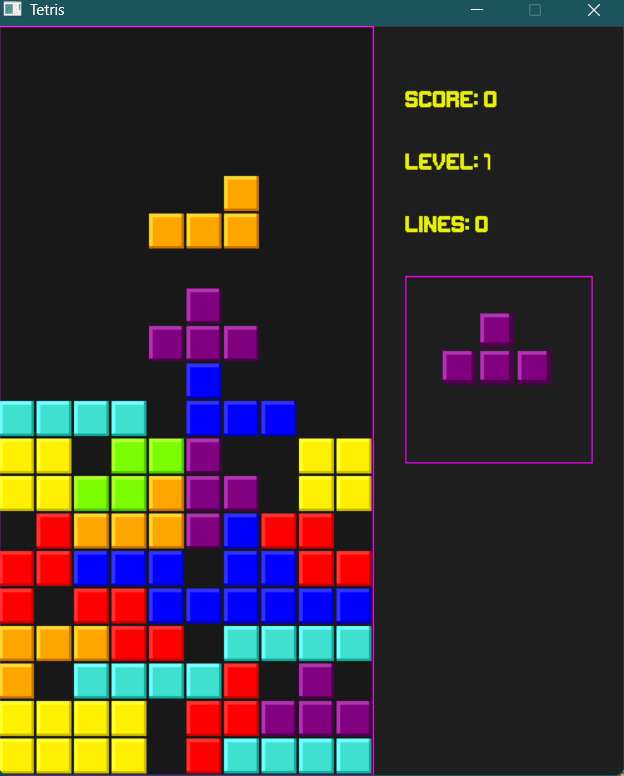
\includegraphics[width=0.5\textwidth]{Figure_1_Tetris.png}
    \\
    \caption{Rendu initial avec proportions \texttt{(7 * size) / 8, size / 8}.}
    \label{fig:figure1}
\end{center}

\begin{center}
    \centering
    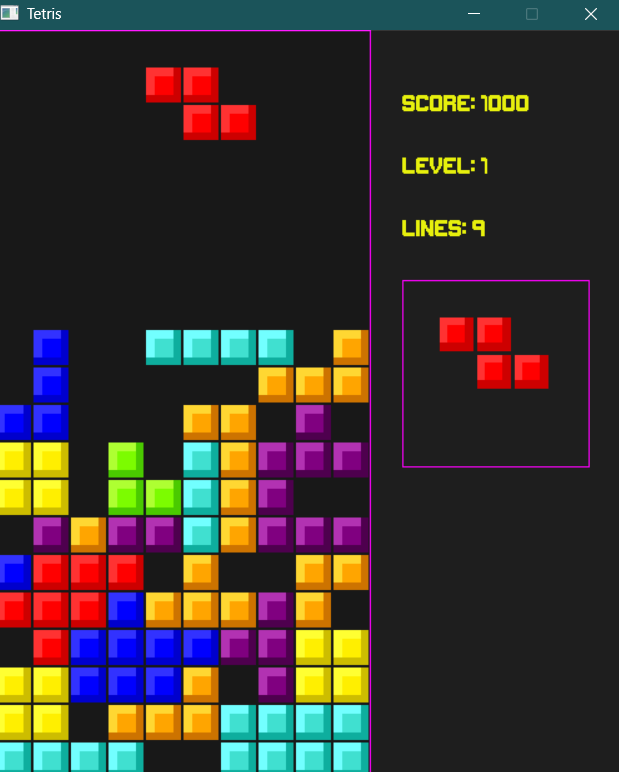
\includegraphics[width=0.5\textwidth]{Figure_2_Tetris.png}
    \\
    \caption{Rendu final avec proportions \texttt{(3 * size) / 4, size / 4}.}
    \label{fig:figure2}
\end{center}
\\
\newpage
\subsection{Ajustements spécifiques des bandes sombre}

Pour améliorer encore le rendu visuel :
\\

Nous avons réduit légèrement les dimensions des bandes sombre en appliquant des décalages (\texttt{-1} et \texttt{-2}) sur leurs coordonnées. Ces ajustements subtils permettent de créer une impression de profondeur accrue sans chevauchement visuel.
\\
\begin{center}
    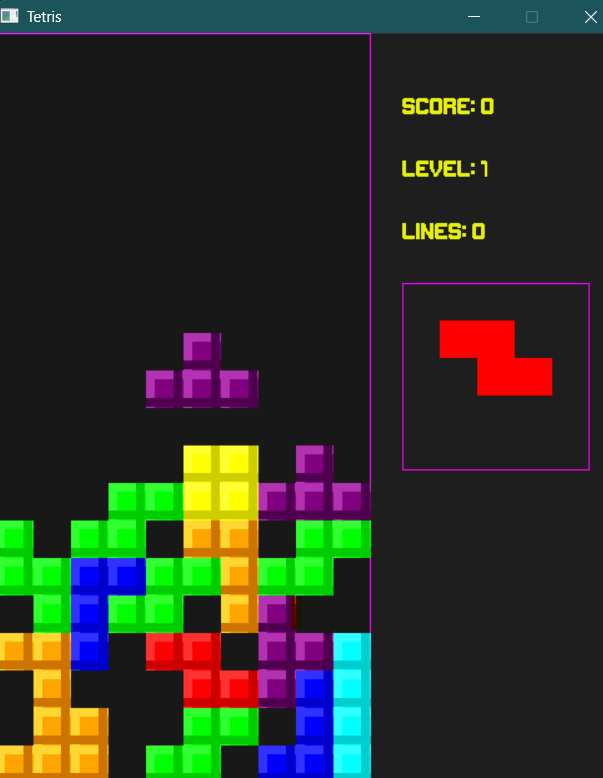
\includegraphics[width=0.7\textwidth]{Figure_3_Tetris.png}
    \\
    \caption{Rendu déséquilibré inspiré de l'exemple mal ajusté.}
    \label{fig:figure3}
\end{center}

\newpage

\chapter{Résultats}

\section{Présentation du jeu final}

Le projet Tetris a été développé en utilisant la bibliothèque SDL pour gérer les graphismes et les entrées utilisateur. Voici une présentation des différentes étapes et fonctionnalités du jeu final :

\subsection{Écran de menu}
Lorsque le jeu est lancé, le joueur est accueilli par un écran de menu. Celui-ci affiche le titre du jeu, des instructions, et une option pour commencer la partie en appuyant sur la touche \texttt{ESPACE} ou \texttt{ENTRÉE}.

\begin{center}
    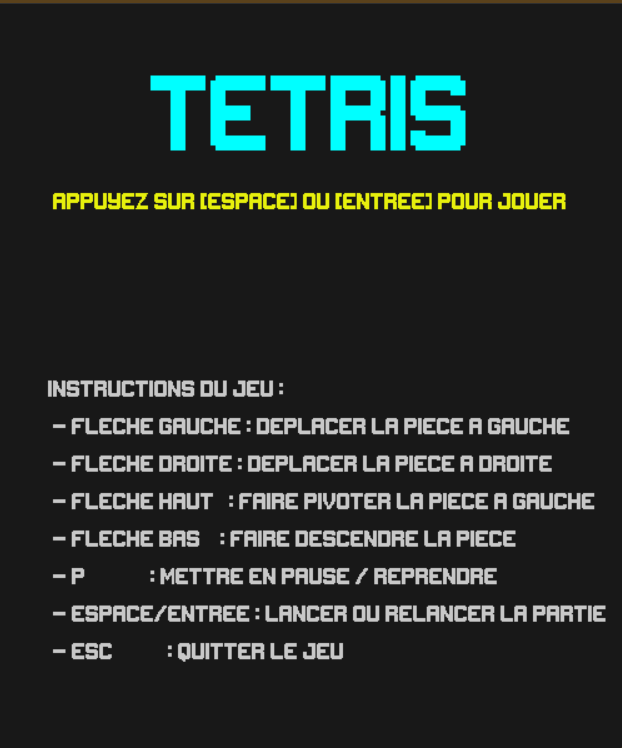
\includegraphics[width=0.5\textwidth]{Figure_Menu.png}
    \\
    \caption{Écran de menu du jeu Tetris}
    \label{fig:menu}
\end{center}

\subsection{En jeu}
Pendant la partie, le joueur peut contrôler les Tetriminos à l'aide des flèches directionnelles pour les déplacer ou les faire pivoter. Le score, le niveau, et le nombre de lignes détruites sont affichés sur le côté droit de l'écran. Le prochain Tetrimino est également prévisualisé pour aider le joueur à planifier ses mouvements.

\begin{center}
    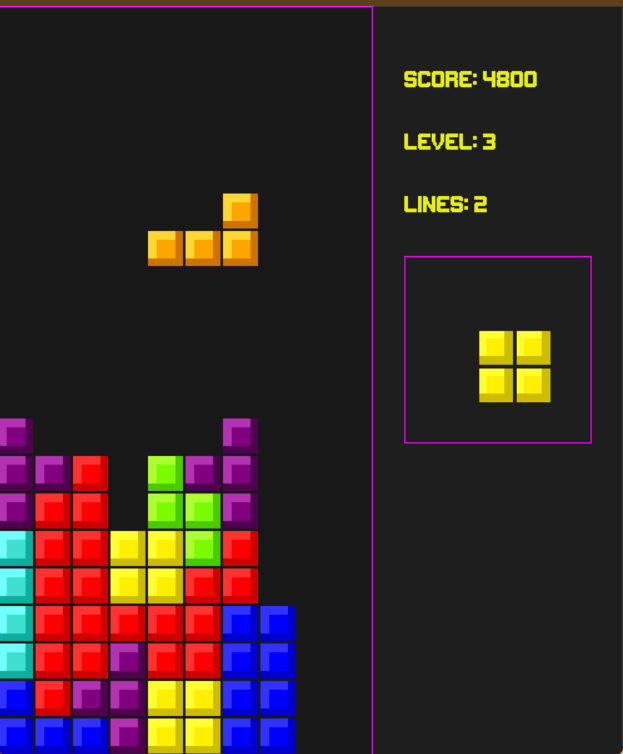
\includegraphics[width=0.8\textwidth]{Figure_jeu.png}
    \\
    \caption{Écran principal en cours de partie}
    \label{fig:gameplay}
\end{center}

\newpage
\subsection{Pause}
Le joueur peut mettre la partie en pause à tout moment en appuyant sur la touche \texttt{P}. Un écran de pause s'affiche alors avec des instructions pour reprendre la partie.

\begin{center}
    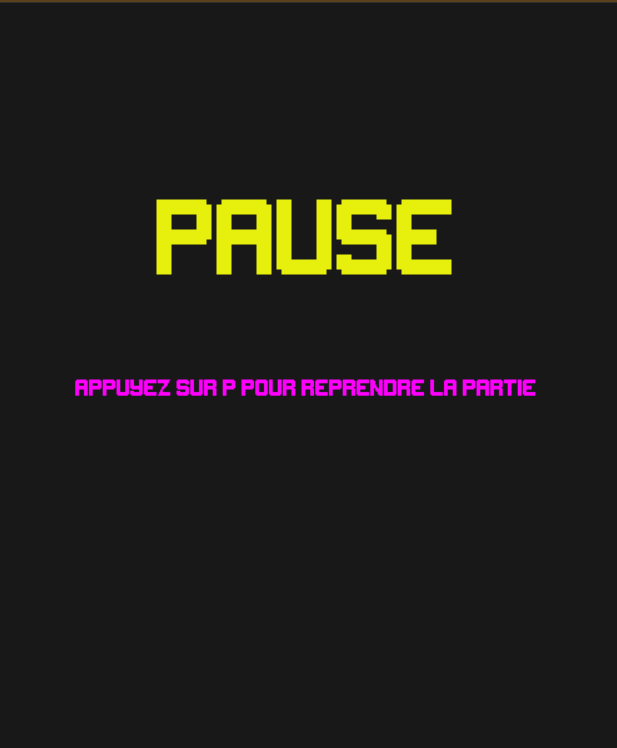
\includegraphics[width=0.8\textwidth]{Figure_Pause.png}
    \\
    \caption{Écran de pause du jeu Tetris}
    \label{fig:pause}
\end{center}

\newpage
\subsection{Fin de partie}
Lorsque les blocs atteignent le sommet du plateau, la partie est terminée. Un écran de Game Over s'affiche, indiquant le score final, le niveau atteint, et le nombre de lignes détruites.

\begin{center}
    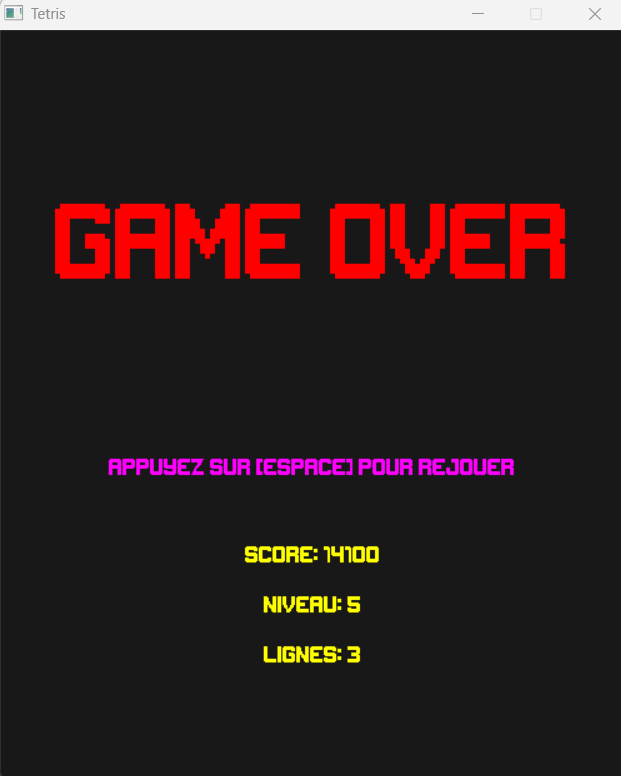
\includegraphics[width=0.8\textwidth]{Figure_Game_Over.png}
    \\
    \caption{Écran de fin de partie (Game Over)}
    \label{fig:gameover}
\end{center}


\newpage

\section{Limites et aspects à améliorer}

Bien que le jeu soit fonctionnel et respecte les exigences initiales du projet, certaines limites et améliorations potentielles ont été identifiées :

\subsection{Limites actuelles}
\begin{itemize}
    \item \textbf{Manque de modes de jeu :} Le jeu se limite à un mode solo classique sans variation.
    \item \textbf{Graphismes simples :} Bien que fonctionnels, les graphismes pourraient être améliorés avec des animations ou des effets visuels.
    \item \textbf{Absence de sauvegarde :} Le jeu ne propose pas de sauvegarde du score ou d’historique des parties.
    \item \textbf{Gestion sonore basique :} Les sons sont simples et pourraient être enrichis par des effets plus variés ou une bande-son personnalisée.
\end{itemize}

\subsection{Propositions d'amélioration}
\begin{itemize}
    \item \textbf{Ajout de modes de jeu :} Implémenter des modes supplémentaires comme un mode contre-la-montre ou un mode multijoueur local.
    \item \textbf{Animations visuelles :} Ajouter des animations pour la rotation des Tetriminos.
    \item \textbf{Niveaux de difficulté :} Proposer des options pour ajuster la difficulté, comme un mode débutant ou expert.
    \item \textbf{Sauvegarde des scores :} Créer un tableau des meilleurs scores pour encourager la rejouabilité.
\end{itemize}


\newpage
\chapter{Conclusion}

Le développement de ce projet Tetris a permis de mettre en pratique des compétences clés en programmation C, en gestion de projets logiciels, et en utilisation de la bibliothèque SDL pour les graphismes et les entrées utilisateur. À travers les différentes étapes de conception et d'implémentation, de nombreux défis ont été relevés, allant de la gestion des collisions à l'affichage graphique, en passant par la détection des états de jeu comme le Game Over.
\\

Le résultat final est un jeu fonctionnel respectant les règles classiques de Tetris. Il inclut des fonctionnalités telles que le calcul du score, l'affichage du prochain Tetrimino, et la progression des niveaux. Ces éléments offrent une expérience utilisateur fluide et fidèle au concept original.
\\

Cependant, certaines limitations subsistent, comme l'absence de modes de jeu alternatifs, des graphismes simples, et l'absence de fonctionnalités de sauvegarde ou de personnalisation. Ces aspects pourraient être développés dans le futur pour enrichir l'expérience utilisateur et améliorer la qualité globale du projet.
\\

Ce projet a non seulement permis de créer un jeu, mais il a également constitué une excellente opportunité d'apprentissage et de perfectionnement. Il a renforcé les compétences en algorithmique, en gestion mémoire, et en programmation événementielle, tout en offrant une perspective concrète sur la création d’un jeu vidéo. Avec des améliorations futures, ce projet pourrait devenir une version encore plus aboutie et moderne du Tetris classique.
\\


\newpage


\chapter{Références}

\textbf{Font Tetris :}  
\\
\url{https://www.dafont.com/fr/gameplay.font?text=TETRIS}

\vspace{0.5cm}

\textbf{Musique de fond :}  
\\
\url{https://www.youtube.com/watch?v=NmCCQxVBfyM}

\vspace{0.5cm}

\textbf{Musique pour l'état Pause :}  
\\
\url{https://www.youtube.com/watch?v=9TPazxfqVLk}

\vspace{0.5cm}

\textbf{Son joué lors du Game Over :}  
\\
1\textsuperscript{er} son dans la vidéo : \url{https://www.youtube.com/watch?v=bug1b0fQS8Y}

\vspace{0.5cm}

\textbf{Son joué lorsque des lignes sont détruites :}  
\\
4\textsuperscript{ème} son dans la vidéo : \url{https://www.youtube.com/watch?v=VhHJomZDpbA}

\vspace{0.5cm}

\textbf{Son joué lorsqu'on passe un niveau :}  
\\
\url{https://www.youtube.com/watch?v=qvBteOqddqk}

\vspace{0.5cm}

\textbf{Son joué lorsque le Tetrimino atterrit :}  
\\
Fait par nous en frappant deux bouteilles en verre.



\end{document}
